\documentclass[12pt,titlepage]{article}
\usepackage[margin=1.25in]{geometry}
\usepackage{graphicx,amsmath,blindtext,minted}

%% Variables definition
\newcommand{\vSubject}{Object Oriented Programming}
\newcommand{\vSubtitle}{Quiz 2}
\newcommand{\vName}{Dicha Zelianivan Arkana}
\newcommand{\vNIM}{2241720002}
\newcommand{\vClass}{2i}
\newcommand{\vDepartment}{Information Technology}
\newcommand{\vStudyProgram}{D4 Informatics Engineering}

%% [START] Tikz related stuff
\usepackage{tikz}
\usetikzlibrary{svg.path,calc,shapes.geometric,shapes.misc}
\tikzstyle{terminator} = [rectangle, draw, text centered, rounded corners = 1em, minimum height=2em]
\tikzstyle{preparation} = [chamfered rectangle, chamfered rectangle sep=0.75em, draw, text centered, minimum height = 2em]
\tikzstyle{process} = [rectangle, draw, text centered, minimum height=2em]
\tikzstyle{decision} = [diamond, aspect=2, draw, text centered, minimum height=2em]
\tikzstyle{data}=[trapezium, draw, text centered, trapezium left angle=60, trapezium right angle=120, minimum height=2em]
\tikzstyle{connector} = [line width=0.25mm,->]
%% [END] Tikz related stuff

%% [START] Fancy header related stuff
\usepackage{fancyhdr}
\pagestyle{fancy}
\setlength{\headheight}{15pt} % compensate fancyhdr style
\fancyhead{}
\fancyfoot{}
\fancyfoot[L]{\thepage}
\fancyfoot[R]{\textit{\vSubject - \vSubtitle}}
\renewcommand{\footrulewidth}{0.4pt}% default is 0pt, overline for footer
%% [END] Fancy header related stuff

%% [START] Custom tabular command related stuff
\usepackage{tabularx}
\newcommand{\details}[2]{
    #1 & #2  \\
}
%% [END] Custom tabular command related stuff

%% [START] Figure related stuff
\newcommand{\image}[3][1]{
    \begin{figure}[h]
        \centering
        \includegraphics[#1]{#2}
        \caption{#3}
        \label{#3}
    \end{figure}
}
%% [END] Figure related stuff

\begin{document}
\begin{titlepage}
    \centering
    \vfill
    {\bfseries\LARGE
        \vSubject\\
        \vskip0.25cm
        \vSubtitle
    }
    \vfill
    
\includegraphics[width=6cm]{images/polinema-logo.png}
    \vfill
    {
        \textbf{Name}\\
        \vName\\
        \vskip0.5cm
        \textbf{NIM}\\
        \vNIM\\
        \vskip0.5cm
        \textbf{Class}\\
        \vClass\\
        \vskip0.5cm
        \textbf{Department}\\
        \vDepartment\\
        \vskip0.5cm
        \textbf{Study Program}\\
        \vStudyProgram
    }
\end{titlepage}

\section{Quiz 2}

\begin{enumerate}
    \item {
        \texttt{Mahasiswa.java}
        \begin{minted}[autogobble,fontsize=\small]{java}
            import java.util.List;

            public class Mahasiswa {
                private String nama;
                private int nim;
                private List<Double> daftarNilai;

                public Mahasiswa(String nama, int nim, List<Double> daftarNilai) {
                    this.nama = nama;
                    this.nim = nim;
                    this.daftarNilai = daftarNilai;
                }

                public String getNama() {
                    return nama;
                }

                public void setNama(String nama) {
                    this.nama = nama;
                }

                public int getNim() {
                    return nim;
                }

                public void setNim(int nim) {
                    this.nim = nim;
                }

                public List<Double> getDaftarNilai() {
                    return daftarNilai;
                }

                public void setDaftarNilai(List<Double> daftarNilai) {
                    this.daftarNilai = daftarNilai;
                }

                public double calculateNilai() {
                    double total = 0;
                    for (int i = 0; i < daftarNilai.size(); i++) {
                        total += daftarNilai.get(i);
                    }
                    return total / daftarNilai.size();
                }

                public double calculateNilai(int[] bobot) {
                    if (daftarNilai.size() != bobot.length) {
                        throw new IllegalArgumentException("Jumlah nilai dan bobot tidak sama");
                    }
                    double total = 0;
                    double totalBobot = 0;
                    for (int i = 0; i < daftarNilai.size(); i++) {
                        total += daftarNilai.get(i) * bobot[i];
                        totalBobot += bobot[i];
                    }
                    return total / totalBobot;
                }
            }
        \end{minted}
    }
    \item {
        \texttt{MataKuliah.java}
        \begin{minted}[autogobble,fontsize=\small]{java}
            import java.util.List;

            public class MataKuliah {
                private String nama;
                private double sks;
                private List<Double> daftarNilaiMahasiswa;

                public MataKuliah(String nama, double sks, List<Double> daftarNilaiMahasiswa) {
                    this.nama = nama;
                    this.sks = sks;
                    this.daftarNilaiMahasiswa = daftarNilaiMahasiswa;
                }

                public String getNama() {
                    return nama;
                }

                public void setNama(String nama) {
                    this.nama = nama;
                }

                public double getSks() {
                    return sks;
                }

                public void setSks(double sks) {
                    this.sks = sks;
                }

                public List<Double> getDaftarNilaiMahasiswa() {
                    return daftarNilaiMahasiswa;
                }

                public void setDaftarNilaiMahasiswa(List<Double> daftarNilaiMahasiswa) {
                    this.daftarNilaiMahasiswa = daftarNilaiMahasiswa;
                }

                public double calculateBobot() {
                    double total = 0;
                    for (Double aDouble : daftarNilaiMahasiswa) {
                        total += aDouble;
                    }
                    return total / daftarNilaiMahasiswa.size();
                }

                public double calculateBobot(List<Double> bobot) {
                    if (daftarNilaiMahasiswa.size() != bobot.size()) {
                        throw new IllegalArgumentException("Jumlah nilai dan bobot tidak sama");
                    }
                    double total = 0;
                    double totalBobot = 0;
                    for (int i = 0; i < daftarNilaiMahasiswa.size(); i++) {
                        total += daftarNilaiMahasiswa.get(i) * bobot.get(i);
                        totalBobot += bobot.get(i);
                    }
                    return total / totalBobot;
                }
            }
        \end{minted}
    }
    \item {
        \texttt{Perwalian.java}
        \begin{minted}[autogobble,fontsize=\small]{java}
            import java.util.List;

            public class Perwalian {
                private List<Mahasiswa> daftarMahasiswa;
                private List<MataKuliah> daftarMataKuliah;

                public Perwalian(
                    List<Mahasiswa> daftarMahasiswa,
                    List<MataKuliah> daftarMataKuliah
                ) {
                    this.daftarMahasiswa = daftarMahasiswa;
                    this.daftarMataKuliah = daftarMataKuliah;
                }

                public List<Mahasiswa> getDaftarMahasiswa() {
                    return daftarMahasiswa;
                }

                public void setDaftarMahasiswa(List<Mahasiswa> daftarMahasiswa) {
                    this.daftarMahasiswa = daftarMahasiswa;
                }

                public List<MataKuliah> getDaftarMataKuliah() {
                    return daftarMataKuliah;
                }

                public void setDaftarMataKuliah(List<MataKuliah> daftarMataKuliah) {
                    this.daftarMataKuliah = daftarMataKuliah;
                }

                public void displayDaftarMahaSiswa() {
                    for (int i = 0; i < daftarMahasiswa.size(); i++) {
                        Mahasiswa mahasiswa = daftarMahasiswa.get(i);
                        MataKuliah mataKuliah = daftarMataKuliah.get(i);

                        System.out.println(
                            "Mahasiswa: " + mahasiswa.getNama() + 
                            ", NIM: " + mahasiswa.getNim()
                        );
                        System.out.println(
                            "Nilai Mahasiswa: " + mataKuliah.getDaftarNilaiMahasiswa()
                        );
                        System.out.println("Bobot Mata Kuliah: " + mataKuliah.calculateBobot());
                        System.out.println();
                    }
                }
            }
        \end{minted}
    }
    \item {
        \texttt{Main.java}
        \begin{minted}[autogobble,fontsize=\small]{java}
            import java.util.List;

            public class Main {
                public static void main(String[] args) {
                    List<Double> daftarNilai1 = List.of(3.4, 3.5, 3.6);
                    List<Double> daftarNilai2 = List.of(3.4, 3.5, 3.6);
                    List<Double> daftarNilai3 = List.of(3.4, 3.5, 3.6);

                    Mahasiswa mahasiswa1 = new Mahasiswa("Andi", 123, daftarNilai1);
                    Mahasiswa mahasiswa2 = new Mahasiswa("Budi", 456, daftarNilai2);
                    Mahasiswa mahasiswa3 = new Mahasiswa("Candra", 789, daftarNilai3);

                    List<Mahasiswa> daftarMahasiswa = List.of(
                        mahasiswa1,
                        mahasiswa2,
                        mahasiswa3
                    );

                    MataKuliah mataKuliah1 = new MataKuliah(
                        "Pemrograman Berorientasi Objek", 3, daftarNilai1
                    );
                    MataKuliah mataKuliah2 = new MataKuliah(
                        "Pemrograman Web", 3, daftarNilai2
                    );
                    MataKuliah mataKuliah3 = new MataKuliah(
                        "Basis Data", 3, daftarNilai3
                    );

                    List<MataKuliah> daftarMataKuliah = List.of(
                        mataKuliah1,
                        mataKuliah2,
                        mataKuliah3
                    );

                    Perwalian perwalian = new Perwalian(daftarMahasiswa, daftarMataKuliah);

                    System.out.println("Daftar Mahasiswa");
                    perwalian.displayDaftarMahaSiswa();
                }
            }
        \end{minted}
    }
    \pagebreak
    \item {
        \texttt{Output}\\
        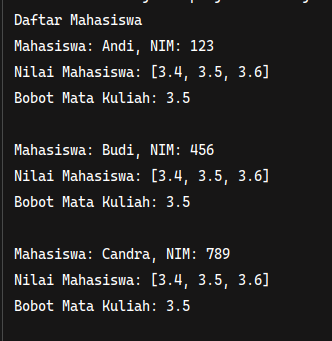
\includegraphics[height=8cm]{./images/output.png}
    }
\end{enumerate}

\end{document}

